\documentclass[conference]{IEEEtran}
\usepackage{amsmath,graphicx,booktabs}
\title{Mobility-Aware and Deadline-Constrained LoRa Communication for UAV Missions: A Simulation Framework}
\author{\IEEEauthorblockN{Lalit Kumar}\IEEEauthorblockA{Robotics and Automation, MANIT Bhopal, India}}
\begin{document}
\maketitle
\begin{abstract}
LoRa enables long-range low-rate robotic telemetry, yet packet reception is not equivalent to fresh status or on-time safety alerts. We specify MARS-LoRa, a seeded simulation comparing fixed spreading factor, link-reactive adaptation, priority-aware scheduling, and a conservative mission slowdown policy. We evaluate application delivery, alert deadline satisfaction, age of information, outage duration, and transmission-energy proxy under mobility and shadowing. This study proceeds from 720 seeded abstract-channel trials and 1,440 factorial ablations to native MuJoCo-executed quadrotor trajectories and a 240-trial comparison of shortest-safe versus RF-aware 3-D routes. The proposed route planner uses a prior static occupancy map and a synthetic, not field-calibrated, LoRa model. Additional held-out propagation tests show that the extra RF detour offers negligible delivery benefit under adequate coverage and can harm critical-alert timeliness under interference. A 40-case deterministic native wind sweep also exposes controller failures and unsafe clearances. GPS-denied navigation and hardware radio validation remain outstanding.
\end{abstract}
\begin{IEEEkeywords}LoRa, UAV, robotics, age of information, timely telemetry\end{IEEEkeywords}
\section{Introduction}
Robotic operations require more than eventual packet delivery. LoRa trades low-power range for transmission airtime, so long packets and weak links may compromise deadline-sensitive information \cite{bor,centenaro}. Age of Information (AoI) captures the freshness of received status \cite{kaul}. This paper asks how communication adaptation and mission-duration overhead influence critical alert timeliness under mobility. We contribute a reproducible simulator, explicit policy baselines, and a test protocol rather than an unverified improvement claim.
\begin{figure}[t]
\centering\fbox{\begin{minipage}{0.92\linewidth}\centering\small
UAV inspection trajectory / MuJoCo pose interface\\[2pt]
$\downarrow$ position, velocity, obstruction\\[2pt]
\fbox{Raw-LoRa channel + message queue}\\[2pt]
$\updownarrow$ telemetry, alerts, RSSI feedback\\[2pt]
\fbox{Fixed / Reactive / Priority / MARS policies}\\[2pt]
$\downarrow$ seeded event log\\[2pt]
CSV metrics $\rightarrow$ figures $\rightarrow$ manuscript / dashboard
\end{minipage}}
\caption{Reproducible research architecture. The original baseline uses kinematic motion; additional controlled experiments use real MuJoCo physics traces, while ROS 2 remains an experimental interface.}\label{fig:arch}
\end{figure}
\section{Related Work and Scope}
LoRa spreading factor changes sensitivity and airtime \cite{bor}; LoRaWAN adds network procedures not included here \cite{centenaro}. We model raw point-to-point LoRa, not LoRaWAN. MuJoCo \cite{todorov} supports the native physical flight traces used in later sections; ROS 2 \cite{macenski} is an experimental integration path. The first controlled channel baseline remains kinematic, and none of the experiments constitute a physical-airframe or radio field test.
\section{Mission and Link Model}
A single UAV follows a high-loss urban (path-loss exponent 4) rectangular 900-m inspection route around a fixed ground station. Nominal speeds are 2, 5, and 9 m/s; timestep is 0.5 s. A designated shadowing region introduces 17 dB obstruction. Routine messages expire after 8 s; critical alerts generated every 45 s expire after 3 s.
Received power in dBm follows
\begin{equation}P_r=14-31.2-40\log_{10}(\max\{1,d\})-L_{obs}+X_t.\end{equation}
Here distance $d$ is in metres, $L_{obs}\in\{0,17\}$ dB, and correlated Gaussian shadowing satisfies
\begin{equation}X_t=0.96X_{t-1}+\sqrt{1-0.96^2}\epsilon_t,\quad\epsilon_t\sim\mathcal N(0,\sigma^2).\end{equation}
We study $\sigma\in\{1,4,8\}$ dB. SF7--SF12, 125 kHz bandwidth, coding rate 4/5, explicit header, and CRC determine transmitter airtime. Success probability uses an SF-dependent sensitivity sigmoid multiplied by 0.9 synthetic occupancy. This factor is not a realistic co-channel collision model; SF changes assume instantaneous receiver coordination. Estimated TX energy is $0.12\sum_i T_{air,i}$ joules, excluding flight and receiver energy.
\section{Policies and Hypotheses}
B1 fixes SF9 and transmits routine telemetry every 2 s. B2 selects the lowest SF satisfying a 6-dB sensitivity margin based on prior acknowledged RSSI, with the same interval. B3 adds critical-first queueing and reduces routine traffic to every 3 s. MARS limits SF changes to one step per decision, uses priority queueing, sends routine telemetry every 4 s, and slows the full mission to 80 percent of nominal speed. The latter is a conservative prototype, not yet a predicted-link-driven maneuver selector. The differing traffic rates confound comparisons; ablation is required to attribute causality. We hypothesize that timeliness and AoI can reveal tradeoffs hidden by overall delivery.
\section{Reproducible Experiments}
Four policies, three speeds, three shadow intensities, and 20 trial seeds yield 720 planned trials. The simulator exports trial-level and grouped CSVs. Application delivery fraction is received/generated. Critical deadline satisfaction is timely critical deliveries divided by generated critical alerts. For newest received creation time $u(t)$, freshness age is $\Delta(t)=t-u(t)$. An outage counts when more than 15 s pass without delivery. Additional outcomes are mean and trial-level 95th-percentile AoI, airtime, estimated TX energy, and mission duration. Pairing the RNG seeds does not enforce identical spatial fading across differently paced missions; a spatial common-random field is future work.
\section{Results and Discussion}
All 720 seeded event-based simulation trials completed in the GitHub Actions workflow. The tabulated values are measured outputs of the \emph{synthetic simulator}, not real radio measurements. For the 2 m/s, 4 dB-shadowing scenario, Table~\ref{tab:example} shows descriptive mean values across 20 trials. No statistical significance is inferred.
\begin{table}[t]\centering\caption{Synthetic model trial means: 2 m/s, $\sigma=4$ dB; $n=20$ seeds.}\label{tab:example}
\begin{tabular}{lrrr}\toprule
Policy & App. delivery & Alert on time & AoI P95 (s)\\\midrule
Fixed SF9 & 0.585 & 0.507 & 57.3\\
Reactive SF & 0.675 & 0.614 & 49.0\\
Priority-aware & 0.629 & 0.643 & 77.8\\
MARS prototype & 0.673 & 0.600 & 66.3\\
\bottomrule\end{tabular}\end{table}
The priority-aware baseline has the greatest mean alert deadline satisfaction in this illustrative scenario (0.643), not MARS (0.600). Reactive SF produces the highest mean application delivery (0.675), marginally above MARS (0.673). MARS also extends mission time from 360 to 450 s by design. These differences cannot isolate SF adjustment, packet interval, or slowdown effects, because policy settings vary simultaneously. Moreover, a longer run generates more alert events. The initial evidence does \emph{not} justify declaring MARS superior.
Figures are generated directly from the saved summary CSV and show speed-related patterns at 4 dB shadowing. More rigorous inference requires per-seed paired comparisons, uncertainty intervals, proper event-time AoI integration, and controlled ablations.
\begin{figure}[t]\centering
\IfFileExists{figures/deadline_satisfaction.pdf}{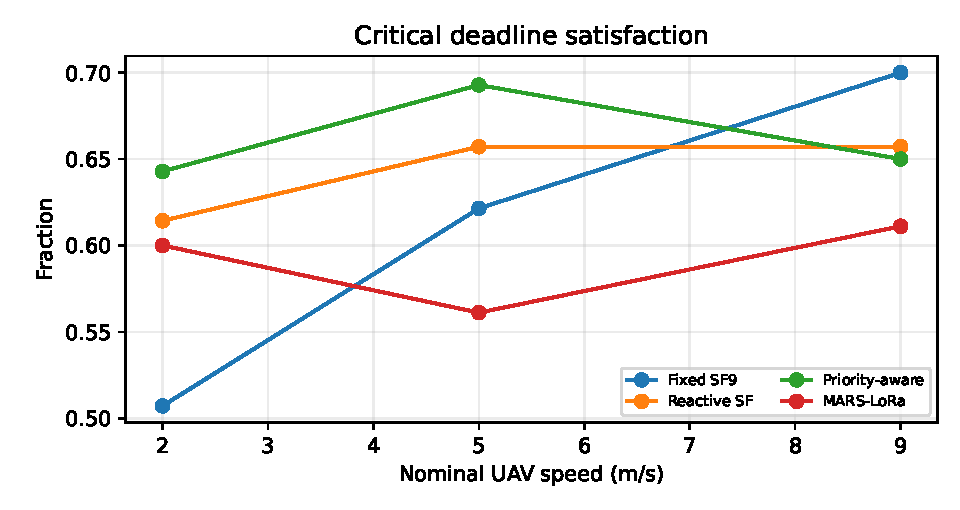
\includegraphics[width=\linewidth]{figures/deadline_satisfaction.pdf}}{\fbox{Deadline plot pending verified run}}
\caption{Critical-alert deadline satisfaction by speed at 4 dB shadowing.}\end{figure}
\begin{figure}[t]\centering
\IfFileExists{figures/aoi_p95.pdf}{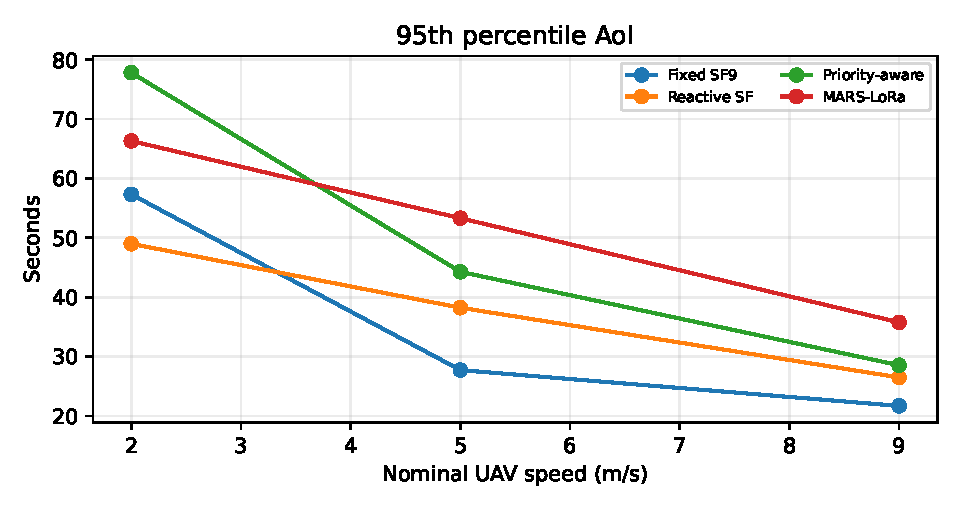
\includegraphics[width=\linewidth]{figures/aoi_p95.pdf}}{\fbox{AoI plot pending verified run}}
\caption{Mean trial-level 95th-percentile AoI at 4 dB shadowing.}\end{figure}
\begin{figure}[t]\centering
\IfFileExists{figures/outage.pdf}{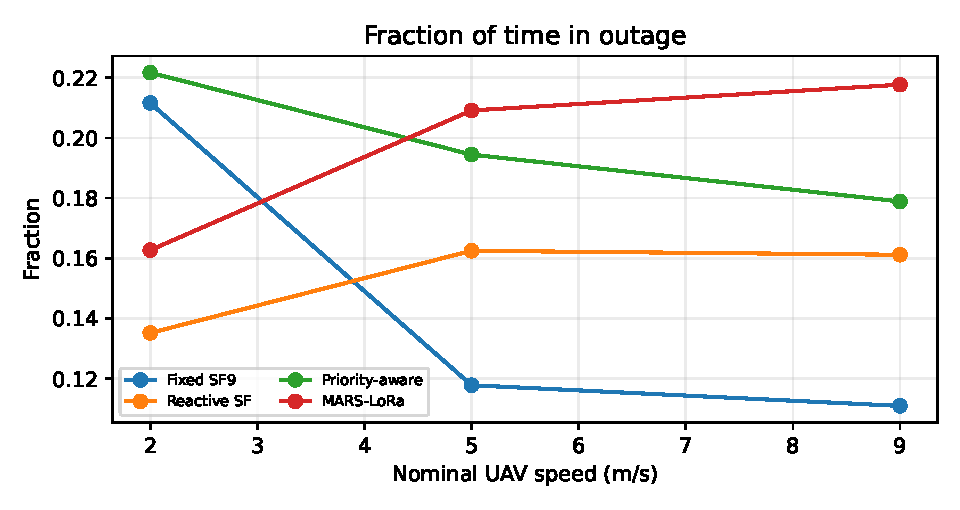
\includegraphics[width=\linewidth]{figures/outage.pdf}}{\fbox{Outage plot pending verified run}}
\caption{Fraction of time without any delivery for over 15 s.}\end{figure}
Interpretation will report critical timeliness jointly with mission overhead and delivery. Longer SF airtime may offset increased weak-signal sensitivity. Negative findings remain publishable when limitations are explicit.
\section{Controlled Factorial Ablation}
We additionally implement a separate $2^3$ factorial experiment with three binary decisions: adaptive SF ($A$), critical-first packet scheduling ($P$), and a conservative 20\% mission-speed reduction ($S$). All eight combinations use a \emph{fixed 2-s telemetry generation interval} and the same 360-s simulation horizon, with time-indexed, seeded fading and receiver draws. Three speeds, three shadowing intensities and 20 seeds give 1,440 executed synthetic-model trials. These ablations reduce traffic-rate and mission-duration confounding in the earlier four-policy study but remain conditional on the simplified radio assumptions.
\begin{table}[t]\centering\caption{Factorial model trial means ($v=2$ m/s, $\sigma=4$ dB, 20 seeds). $A$: SF adaptation; $P$: message priority; $S$: 20\% slowdown.}\label{tab:factorial}
\begin{tabular}{lrrr}\toprule
Variant & Delivery & Alert timely & TX energy (J)\\\midrule
A0P0S0 & .602 & .557 & 4.125\\
A0P1S0 & .602 & .579 & 4.125\\
A1P0S0 & .763 & .793 & 12.255\\
A1P1S0 & .763 & .829 & 12.255\\
A1P1S1 & .734 & .750 & 14.291\\
\bottomrule\end{tabular}\end{table}
For the shown condition, adding adaptive SF with unchanged flight speed and traffic raises mean critical deadline satisfaction from .557 (A0P0S0) to .793 (A1P0S0), but increases the transmitter energy proxy from 4.125 to 12.255 J. With adaptation enabled, the priority factor increases mean timely-alert delivery from .793 (A1P0S0) to .829 (A1P1S0). Adding unconditional slowdown (A1P1S1) \emph{reduces} alert timeliness to .750 while also reducing distance traveled during the fixed window by 20\%. Consequently, unconditional flight slowdown is not an effective strategy in this setting. We report descriptive means, not formal significance claims. Policy effects across the full parameter grid and paired confidence intervals are needed before generalizing.
The adaptive-SF implementation relies on previous ACK-observed RSSI and a bounded five-second slope projection; it assumes the receiver follows all SF changes at no cost, making its gain optimistic. Receiver coordination and an explicitly timed SF handshake are priority corrections before a deployment claim.
\section{GPS-Denied Localization Prototype}
To make waypoint guidance independent of a perfect simulator XY coordinate, we additionally implement a browser-side planar occupancy-mapping and scan-matching prototype. The vehicle carries 32 MuJoCo rangefinder rays distributed over $360^\circ$ with a 25-m range cap; range data are sampled every 0.5 s. A biased odometry proxy integrates body-frame velocity and yaw change. A local discrete scan-to-map search corrects the estimated pose when sufficient occupied endpoints are visible. The waypoint controller can consume this estimated XY position, while onboard attitude stabilization remains local to the simulated vehicle.
The conservative 7-m inspection corridor rises above the highest 5.68-m obstruction and therefore provides almost no horizontal range returns. A separate 3.2-m, geometry-checked landmark survey provides an observable demonstration. Simulated truth is used only for localization error evaluation and the current non-deployable collision supervisor. The map matcher has neither global loop closure nor 6-DoF estimation; camera, inertial bias estimation, range-based onboard safety constraints and validation against ROS 2 SLAM Toolbox \cite{slamtoolbox} remain future tasks. \emph{No quantitative GPS-denied navigation advantage is claimed before repeated physics-and-sensor trials.}
\section{Independent MuJoCo Flight-Physics Check}
We separately evaluated the browser-model MJCF quadrotors in native MuJoCo under one conservative seven-waypoint industrial inspection mission. The plan climbs to 7 m before horizontal transit, clearing the scene's tallest 5.68-m overhead structure, and only descends after returning to the base. It includes deterministic sinusoidal wind forces, linear drag, airframe-specific approximate 45/80-ms motor-response filters, and a velocity-damped position/attitude controller. This experiment is \emph{not} yet integrated into the seeded LoRa communication trials.
\begin{table}[t]\centering
\caption{MuJoCo physics validation; one deterministic mission per vehicle. Contact is checked at every 4-ms physics step. No repeated-seed generalization is claimed.}\label{tab:flight}
\begin{tabular}{lrrr}\toprule
Airframe & Completion (s) & Min. clearance (m) & Contact steps\\\midrule
1.325-kg X2-like & 90.57 & 1.00 & 0\\
27-g Crazyflie-like & 105.35 & 1.24 & 0\\
\bottomrule\end{tabular}\end{table}
Both vehicles completed the deterministic mission with zero MuJoCo contact steps. Their completion times differ under airframe-specific disturbance scaling and actuator response. These traces establish one controlled simulation baseline, not field performance equivalence. A full uncertainty study under random wind, actuator mismatch, sensory delays and multiple obstacle layouts is necessary before asserting robust collision avoidance.
\section{Coupled Flight--Communication Replay}
We next replace the radio-only experiment's prescribed kinematic path with time-stamped poses actually integrated by native MuJoCo for both airframes. A deterministic set of industrial obstacles and 72 generated urban structures is shared with the LoRa propagation proxy. For every sampled UAV-to-receiver segment, a 3-D axis-aligned ray intersection assigns 17 dB excess loss to obstructed links. Both receiver placements lie at $(230,220)$ m, with heights 5 m (ground GCS) or 120 m (elevated relay), producing all-NLOS and mixed-LOS/NLOS episodes, respectively. We combine two airframes, two receivers, two Gaussian shadow levels ($\sigma=4,8$ dB), 20 seeds and three scheduling policies for 480 controlled radio replays. All policies share the same executed flight trace, message generation times and seeded fading; this is physics-conditioned radio evaluation, not yet online RF-aware trajectory adjustment.
\begin{table}[t]\centering\caption{MuJoCo-conditioned raw-LoRa trial means for the 1.325-kg vehicle at 4 dB shadowing ($n=20$ per cell). TX J denotes the proxy $0.12 \sum T_{air}$, not measured transceiver consumption.}\label{tab:crosslayer}
\begin{tabular}{llrrrr}\toprule
Receiver & Radio policy & Delivery & Alert on time & P95 AoI & TX J\\\midrule
Ground & Fixed SF9 & .152 & .217 & 36.86 & 1.08\\
Ground & Adaptive SF & .545 & .467 & 13.44 & 5.82\\
Elevated & Fixed SF9 & .456 & .383 & 26.92 & 1.08\\
Elevated & Adaptive SF & .480 & .400 & 28.98 & 2.14\\
\bottomrule\end{tabular}\end{table}
The demonstrated benefit is conditional on channel geometry: under the fully shadowed ground receiver, SF adaptation greatly improves delivery and freshness but increases radio airtime and the estimated energy proxy about fivefold. At the mixed-LOS/NLOS elevated receiver, adaptation yields a smaller mean delivery gain and a worse mean P95 AoI. A single globally superior policy is not observed. Priority scheduling offers relatively small additional changes with three alerts per approximately 90-s run, so confidence intervals and longer matched tasks are essential before inferring critical-message benefit.
\begin{figure}[t]\centering
\IfFileExists{figures/crosslayer_policies.pdf}{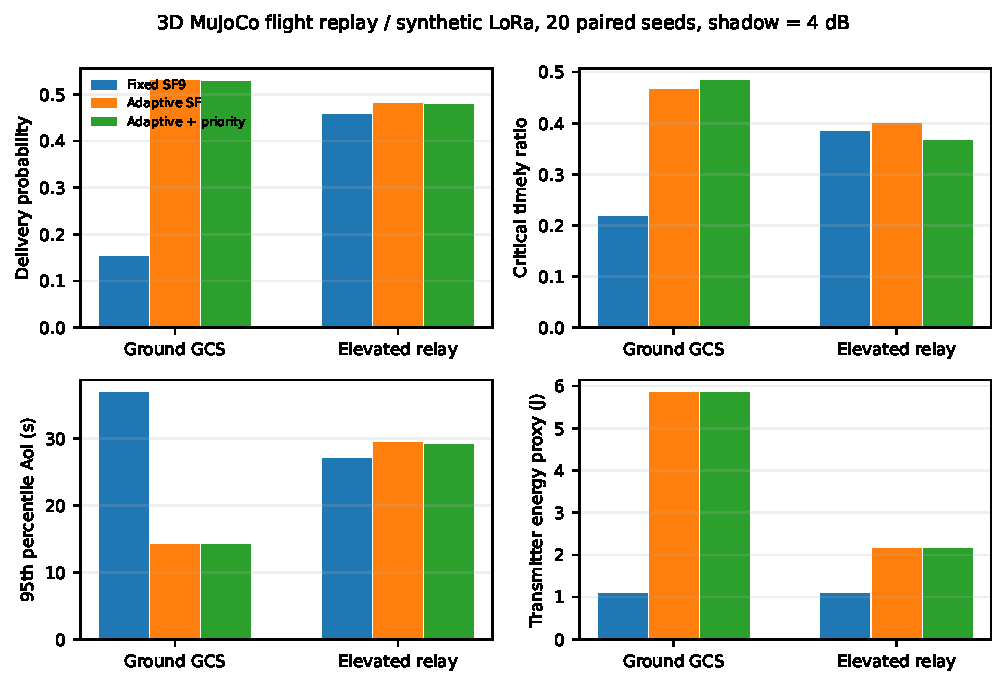
\includegraphics[width=\linewidth]{figures/crosslayer_policies.pdf}}{\fbox{Cross-layer figure pending verified CI run}}
\caption{Reproducible MuJoCo--LoRa policy tradeoffs across urban receiver geometry (4 dB shadowing); generated directly from saved trial CSV.}\end{figure}
Importantly, these simulations still use simplified AABB obstruction, assumed sensitivity thresholds, and stylized SF synchronization. Physics-derived trajectories do not themselves validate propagation. GPS-denied pose estimates have not yet been used to optimize RF-aware flight decisions in this controlled benchmark.
\section{Joint RF-Aware 3D Trajectory Planning}
We next evaluate a map-known, clearance-constrained A* planner \cite{astar} against conventional shortest-safe geometry. The graph spans $3$-m horizontal cells and altitude layers $\{4,7,10,13,17,21,26\}$ m, across the same industrial and seeded urban solids as the native MuJoCo scene. Each candidate edge is sampled at intervals no larger than $0.35$ m and rejected unless signed clearance exceeds the conservative UAV radius plus $0.55$ m. Both planners share start $(0,0,4)$ and goal $(-30,24,4)$ m and optimize a priori before execution. This \emph{assumes a perfect static obstacle map}; it is not an evaluation of onboard SLAM.
For an edge $e$ with length $L_e$ and midpoint $\mathbf{x}_e$, shortest-safe A* minimizes travel length with a 1.4 weight on vertical edges. The RF-aware variant minimizes
\begin{equation}
J(\pi)=\sum_{e\in\pi}\left[L_e\bigl(1+0.4I_{z,e}\bigr)
+4.5L_e\bigl(1-\widehat{P}_{\mathrm{rx}}(\mathbf{x}_e)\bigr)\right],
\end{equation}
subject to the same clearance constraint. Here $\widehat{P}_{\mathrm{rx}}$ is an idealized SF9 reception estimate calculated from ray--box visibility and a distant elevated relay at $(230,220,120)$ m; $I_{z,e}$ indicates a vertical edge. The planner does \emph{not} receive future stochastic fading or packet reception outcomes. We compare (S0) shortest-safe with fixed SF9, (S1) shortest-safe with adaptive SF plus priority scheduling, and (R2) RF-aware routing with the \emph{same} adaptive radio policy. The S1--R2 contrast isolates the added route-planning choice.
\begin{figure}[t]\centering
\IfFileExists{figures/rf_aware_routes.pdf}{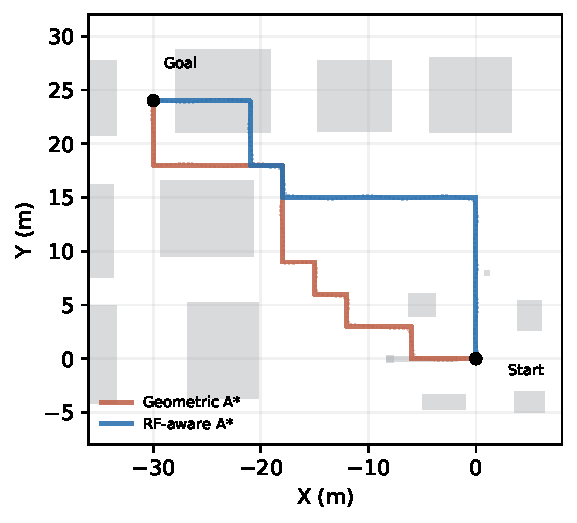
\includegraphics[width=\linewidth]{figures/rf_aware_routes.pdf}}{\fbox{Verified route plot pending CI}}
\caption{Collision-aware 3-D A* route projections and actual MuJoCo tracking. Both methods use identical obstacle geometry; dotted curves are executed flight positions.}\label{fig:rfroute}
\end{figure}
The shortest plan covers 54 m and the RF-aware plan covers 80 m. Their modeled SF9 mean predicted reception along the planned path is 0.046 and 0.712, respectively. All four executed physical trajectories (two aircraft $\times$ two routes) reached the same destination without contact in the deterministic MuJoCo test. For the 1.325-kg model, mission times are 105.23 and 118.51 s, and measured minimum clearances are 0.832 and 1.504 m, respectively. The 27-g vehicle takes 127.08 and 127.36 s, respectively. The path-length increase is a genuine cost; time does not scale proportionally because ascent/descent and waypoint settling dominate.
\begin{table}[t]\centering
\caption{Map-known A* comparison on the 1.325-kg model, $\sigma=4$ dB, $n=20$ matched radio seeds per condition. Values are simulation means.}\label{tab:rfastar}
\begin{tabular}{lrrrr}\toprule
Condition & PDR & Alert timely & P95 AoI (s) & TX J\\\midrule
S0: shortest/fixed & .104 & .050 & 51.78 & 1.25\\
S1: shortest/adaptive & .432 & .500 & 28.56 & 6.29\\
R2: RF route/adaptive & .784 & .838 & 4.33 & 1.35\\
\bottomrule\end{tabular}\end{table}
\begin{figure}[t]\centering
\IfFileExists{figures/rf_aware_tradeoff.pdf}{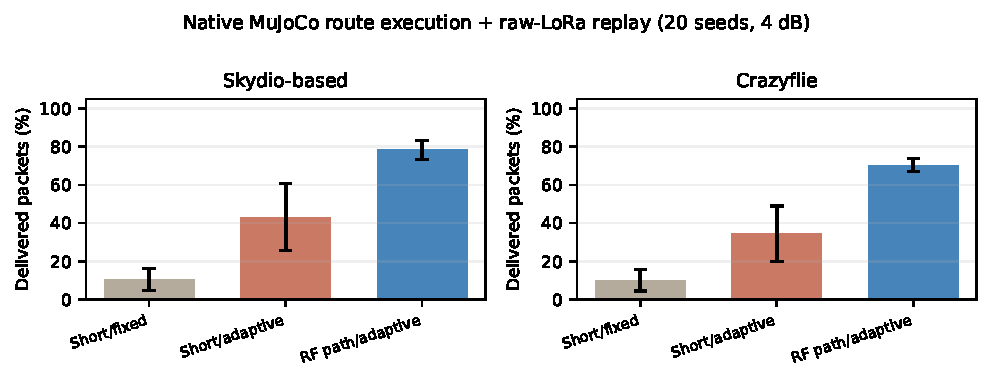
\includegraphics[width=\linewidth]{figures/rf_aware_tradeoff.pdf}}{\fbox{Verified policy plot pending CI}}
\caption{Application delivery with between-trial standard-deviation bars (20 seeded runs, 4 dB shadowing). Not field LoRa reception measurements.}\label{fig:rftrade}
\end{figure}
Relative to S1, R2 improves mean PDR by 0.352 and critical-alert timeliness by 0.338 for the inspection quad, while reducing P95 AoI by 24.24 s and modeled TX energy by 4.93 J. The corresponding paired normal-approximation 95\% confidence interval for PDR difference is [0.271, 0.433], conditional on this one scene and channel model. The path avoids line-of-sight blockage more often, but requires 26 m of additional planned travel and 13.3 s of additional simulated flight. The Crazyflie-derived model also benefits in radio metrics, but this comparison holds routes and modeled radio hardware identical between two airframes rather than testing antenna differences.
These effects are conditional on a \emph{single known map, one relay location, deterministic flight disturbances and a simple ray--AABB radio abstraction}. The initial route trials vary radio fading but not city layout, wind or vehicle sensors; the subsequent held-out tests perturb radio assumptions without changing executed dynamics. Because route duration differs, packet counts and alert opportunities also differ. The resulting estimates should not be interpreted as an independently validated GPS-less or generally optimal control policy.

\section{Held-Out Propagation Stress Test}
The nominal RF-aware plan and shortest plan are \emph{frozen} after their native MuJoCo execution. We then replay each physical trajectory with the same adaptive-priority policy, using 20 paired spatial-fading seeds and five propagation scenarios: nominal shadowing, mild urban loss (path-loss exponent $3.2$, obstruction 9 dB), dense urban loss (exponent $4.4$, obstruction 26 dB), displaced relay and receiver offset, and severe co-channel occupancy (35\%). In this test $X(\mathbf{x})$ is a seeded three-dimensional shadow field constructed by smoothly interpolating Gaussian samples on a spatial grid, so both routes encounter identical attenuation at identical positions even at different times. The interpolated field is continuous but its effective variance is position-dependent; it is not a calibrated spatial covariance model. The changed propagation profiles are \emph{not} provided to the A* planner. This reduces one modeling circularity but does not amount to independent RF validation: both planning and replay still employ a ray--box obstruction surrogate and assumed sensitivity curves.
\begin{figure}[t]\centering
\IfFileExists{figures/heldout_robustness.pdf}{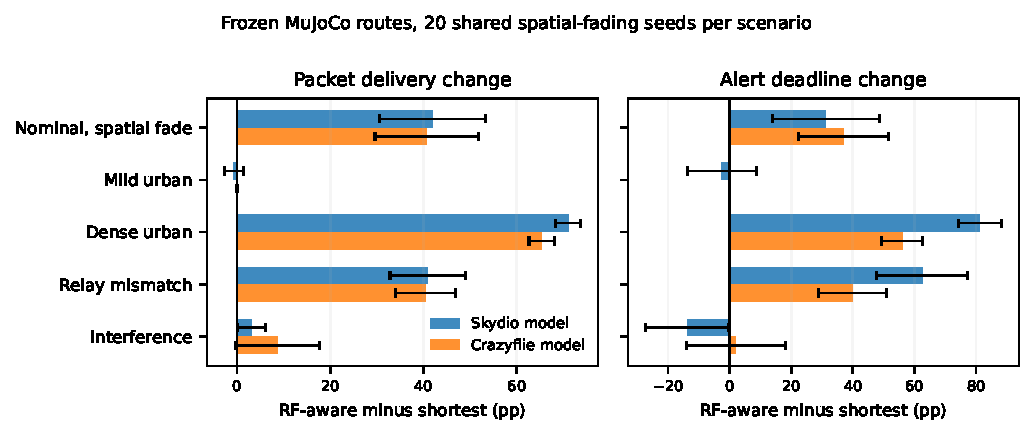
\includegraphics[width=\linewidth]{figures/heldout_robustness.pdf}}{\fbox{Held-out propagation figure pending CI}}
\caption{Route effect across unseen channel settings: RF-aware minus shortest-safe path with identical adaptive LoRa policy; bars show paired normal-approximation 95\% intervals ($n=20$ spatial seeds per profile and vehicle). These intervals do not quantify uncertainty over buildings or hardware.}\label{fig:robustness}
\end{figure}
For the 1.325-kg UAV, the paired improvement in application delivery is 42.0 percentage points under nominal spatial fading (95\% CI 30.6--53.4), but \emph{minus} 0.64 points under mild-urban propagation (95\% CI -2.64--1.36). In that mild case the shortest and RF-aware routes already achieve delivery rates 90.9\% and 90.2\%, respectively, while the detour still requires 13.3 s additional flight. The dense-urban profile favors RF routing by 71.0 points, but at the cost of 6.03 J higher modeled transmitter energy, as adaptation selects slower SF settings. Under high interference the delivery improvement falls to 3.12 points, while \emph{critical-alert deadline satisfaction drops by 13.75 points} (95\% CI -27.27 to -0.23). Thus maximizing predicted packet reception is insufficient for time-constrained robotic communication. A more defensible controller should choose whether to detour based on calibrated expected deadline reliability, flight-time cost, and uncertainty, rather than always favoring the radio-optimized path. These five scenarios are illustrative sensitivity tests, not statistically independent samples of real deployments.

\section{Wind-Disturbance Safety Boundary}
Geometrically collision-free A* routes are insufficient for physically safe autonomous flight. We therefore execute each of the two routes using both airframes at five amplitudes of deterministic sinusoidal force disturbances (0, 0.25, 0.5, 1.0, and 1.5 simulation force-scale units). These are \emph{not} real wind speeds in m/s. Success requires mission completion, zero MuJoCo contacts and measured obstacle clearance at least 0.25 m. The original controller passes 12 of 20 conditions; a higher-authority controller passes 14. Integral correction passes 11, a conservative distance barrier passes 10, and a closing-speed barrier passes 13. None satisfies the full safety requirement. Some failed missions stall, while the Crazyflie-derived model suffers repeated contact at the highest force levels. In one case the new controller completes a flight without contact but breaches the 0.25-m required clearance. We therefore do not promote the higher-authority gains as a safe solution. This deterministic force sweep is not a probability-of-failure estimate; future experiments must independently randomize wind direction, collision geometry and localization error. These failures constrain any claim of reliable LoRa-aware flight.

\section{Joint Route/SF and Propulsion-Energy Caveats}
An exploratory preflight selector uses synthetic RSSI pilots, occupied-channel samples and known 3-D routes to choose a route and fixed SF7--SF12. We evaluate its decisions by replaying actual packet transmissions, not predicted scores. In 200 post-hoc cases a 20\%-of-deadline airtime budget reduces the initial SF12-heavy policy's radio energy, but under high interference the inspection UAV's timely-critical success is only 0.475 versus 0.725 for shortest+adaptive SF. A busy-channel guard (threshold 0.20) falls back to the shortest route and adaptive SF, recovering 0.713, still marginally below baseline. The heuristic thresholds were chosen after inspecting related scenarios, so these results are \emph{not} independent validation.

The original radio-energy analysis overlooks UAV propulsion. Using momentum-theory induced-hover power \cite{hover},
\begin{equation}
P_{\mathrm{ideal}}=\frac{(mg)^{3/2}}{\sqrt{2\rho\,4\pi R^2}},\quad
E_{\mathrm{proxy}}=\frac{P_{\mathrm{ideal}}T}{\eta},
\end{equation}
with assumed $\rho=1.225$ kg/m$^3$, $\eta=0.55$ and \emph{illustrative} rotor radii $R=0.11$ m (1.325-kg craft), $0.023$ m (27-g craft), the 13.28-s detour adds about 1.85 kJ of hover-time electrical proxy for the larger UAV while the modeled LoRa TX saving is 4.93 J (4-dB shadow). Radio-only energy superiority therefore need not imply total mission efficiency. Actual rotor geometry, motor currents and flight aerodynamics are not calibrated.

\section{Unseen-City, Uncertainty-Inflated Evaluation}
To probe geometric overfitting, we froze the experimental route/SF policy and tested two previously unused native MuJoCo city seeds (94103 and 58241; 72 building boxes each) and two additional synthetic propagation profiles. Planning conservatively assumes, but does \emph{not measure}, $\sigma_{\rm loc}=0.10$ m positional uncertainty and adds $3\sigma_{\rm loc}$ to the geometric margin. Each model executes shortest-safe and RF-aware routes with a deterministic low-amplitude force disturbance; any incomplete, contacting or under-clearance flight is counted as a safety failure and excluded from conditional radio comparison. All eight evaluated physical trajectories completed, with no contact and measured minimum clearance $\geq0.90$ m. These deterministic runs do not establish GPS-denied localization or strong-wind robustness.

Across 192 matched-seed synthetic packet trials (two cities, two airframes, two channel profiles, eight radio seeds, three policies), the ex-ante route/SF decision does not consistently dominate shortest-route adaptive SF. In city 58241 with the 1.325-kg craft and displaced relay, timely critical-alert delivery is 0.906 for shortest+adaptive and 0.781 for the joint policy. In city 94103 under stronger shadowing the joint policy yields 0.256 versus 0.219 for shortest+adaptive, but only 0.500 for RF-aware+adaptive. This failure of uniform improvement, together with the larger route's estimated propulsion cost, argues against claiming an optimized or generalizable method. Both maps remain perfectly known and the simulated radio links share a model class; uncertainty is an externally supplied margin, not SLAM-estimated covariance.

\section{GPS-Free Map-Aided LiDAR Correction}
We test whether a known urban map and horizontal range sensing can mitigate the position drift that invalidates a fixed $3\sigma$ clearance assumption. In the physical MuJoCo controller, XY feedback comes from a biased dead-reckoned pose rather than exact simulation truth. The disturbance follows a seeded two-dimensional Brownian walk with diffusion scales $0.03$ and $0.06$ m/$\sqrt{\rm s}$, plus 0.02-m Gaussian measurement noise. A map-aided estimator synthesizes 16 horizontal LiDAR returns (25-m cap, 0.06-m range noise) every 2 s. A bounded coarse-to-fine search corrects the prior XY estimate by minimizing clipped range residuals against the known 3-D boxes at the vehicle's current altitude. Corrections are rejected for insufficient structural returns or inconsistent scans. Position accuracy is scored independently using
\begin{equation}
{\rm ATE}_{xy}=\sqrt{\frac{1}{N}\sum_{k=1}^{N}
\|\hat{\mathbf p}_{xy,k}-\mathbf p_{xy,k}\|^2}.
\end{equation}
In 32 executed paired physical missions (two previously explored cities, two airframes, both A* routes and two drift levels), dead reckoning alone passes 7/8 and 3/8 safety tests, respectively. Map-aided LiDAR matching passes 8/8 at each drift level, reducing mean XY ATE from 0.369 to 0.099 m at $0.03$ and from 1.039 to 0.122 m at $0.06$ m/$\sqrt{\rm s}$. The safety gate requires reaching the target with no MuJoCo contacts and clearance $\geq0.25$ m. The estimator assumes the true orientation, body velocity, altitude, and a perfect obstacle map; it neither builds the map nor estimates IMU biases. These results therefore demonstrate an optimistic GPS-free \emph{map-localization primitive}, \emph{not} verified GPS-denied SLAM. High-altitude horizontal scans may contain too few structures for localization.

\section{Limitations and Deployment}
The channel omits actual radio measurements, antenna orientation, real packet collisions, regulatory duty-cycle scheduling, and control-plane SF handshakes. The first radio baseline uses a kinematic route, while the later cross-layer tests replay independently executed MuJoCo flight traces. The new RF-aware A* planner is a map-known oracle; it does not solve GPS-denied mapping, real-time perception or control under localization uncertainty. A global slowdown is not predictive mobility adaptation. Accordingly, results are hypothesis-generating simulation outcomes, not field evidence. Future validation should compare link predictions against measured LoRa logs, replace ideal map inputs with uncertainty-aware onboard mapping, test varied urban scenes and randomized winds, and close the ROS 2 autonomy loop.
\section{Conclusion}
This open framework makes deadline reliability, freshness, and mission cost jointly measurable for raw-LoRa-linked aerial robots. Its preliminary value is a falsifiable experiment protocol rather than established superiority. Map-known link-predictive 3-D routing now has a reproducible simulation test; future work must validate GPS-denied perception, radio measurements and environmental robustness before any deployment claims.
\begin{thebibliography}{8}
\bibitem{bor} M. Bor et al., ``Do LoRa low-power wide-area networks scale?'' Proc. ACM MSWiM, pp. 59--67, 2016.
\bibitem{centenaro} M. Centenaro et al., ``Long-range communications in unlicensed bands,'' IEEE Wireless Communications, vol. 23, no. 5, pp. 60--67, 2016.
\bibitem{kaul} S. Kaul et al., ``Real-time status: How often should one update?'' Proc. IEEE INFOCOM, pp. 2731--2735, 2012.
\bibitem{todorov} E. Todorov et al., ``MuJoCo: A physics engine for model-based control,'' Proc. IEEE/RSJ IROS, pp. 5026--5033, 2012.
\bibitem{macenski} S. Macenski et al., ``Robot Operating System 2: Design, architecture, and uses in the wild,'' Science Robotics, vol. 7, no. 66, eabm6074, 2022.
\bibitem{slamtoolbox} S. Macenski, ``On Use of SLAM Toolbox: A Fresh(er) Look at Mapping and Localization for the Dynamic World,'' ROSCon, 2019.
\bibitem{astar} P. E. Hart, N. J. Nilsson and B. Raphael, ``A Formal Basis for the Heuristic Determination of Minimum Cost Paths,'' IEEE Trans. Systems Science and Cybernetics, vol. 4, no. 2, pp. 100--107, 1968.
\bibitem{hover} A. M. Perez Gordillo et al., "Numerical and Experimental Estimation of the Efficiency of a Quadcopter Rotor Operating at Hover," Energies, vol. 12, no. 2, article 261, 2019, doi:10.3390/en12020261.
\end{thebibliography}
\end{document}